\chapter{Additional Figures}
\label{chap:additional_figs}

This appendix presents figures for five measures, absolute and relative
netgain, absolute and relative netsnow, and deaggregation factor, that are used
and described in Chapter \ref{chap:analysis}. These figures present the change
in these measures following CIDR Report appearances in the treatment group and
constructed ``appearances'' in the control group, for the four three-year time
periods within the larger study period: 1998-2000, 2001-2003, 2004-2006, and
2007-2009. The purpose of these figures, which did not fit in the main section
of the thesis, are to illustrate the change in these measures in the treatment
and control groups over the study period.

%%%%%%%%%%%%%%%%%%%%%%%%%%%%%%%%%%%%%%%%%%%%%%%%%%%%%%%%%%%%%%%%%%%%%%%%%%%%%%%%
\clearpage
\section{Absolute netgain}

\begin{figure}[H]
\begin{centering}
\begin{singlespace}
\captionsetup{list=no}
    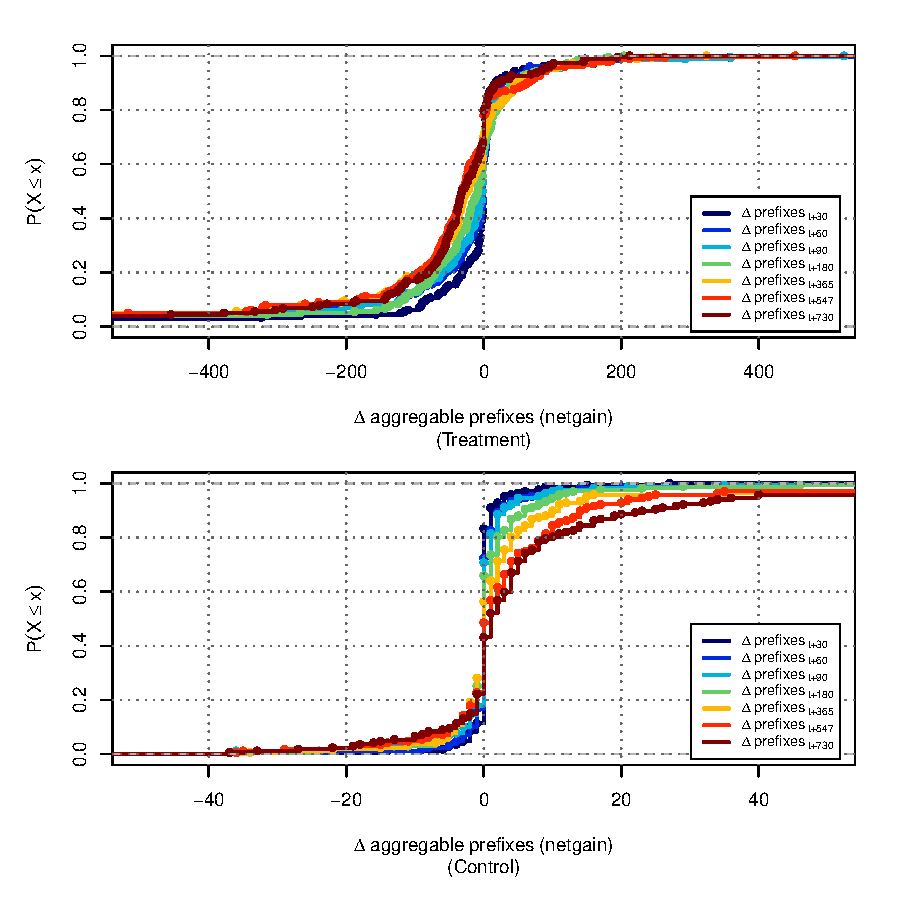
\includegraphics[width=6in]{figures/behavior-netgain-1998_2000-corr.pdf}
    \vspace{-2em}\\
    \caption{Cumulative distribution function of change in number ofaggregable
    prefixes (netgain) advertised by treated and untreated(control) ASes, for
    the period 1998-2000.}
\end{singlespace}
\end{centering}
\end{figure}

\clearpage
\vspace*{16pt}
\begin{figure}[H]
\begin{centering}
\begin{singlespace}
\captionsetup{list=no}
    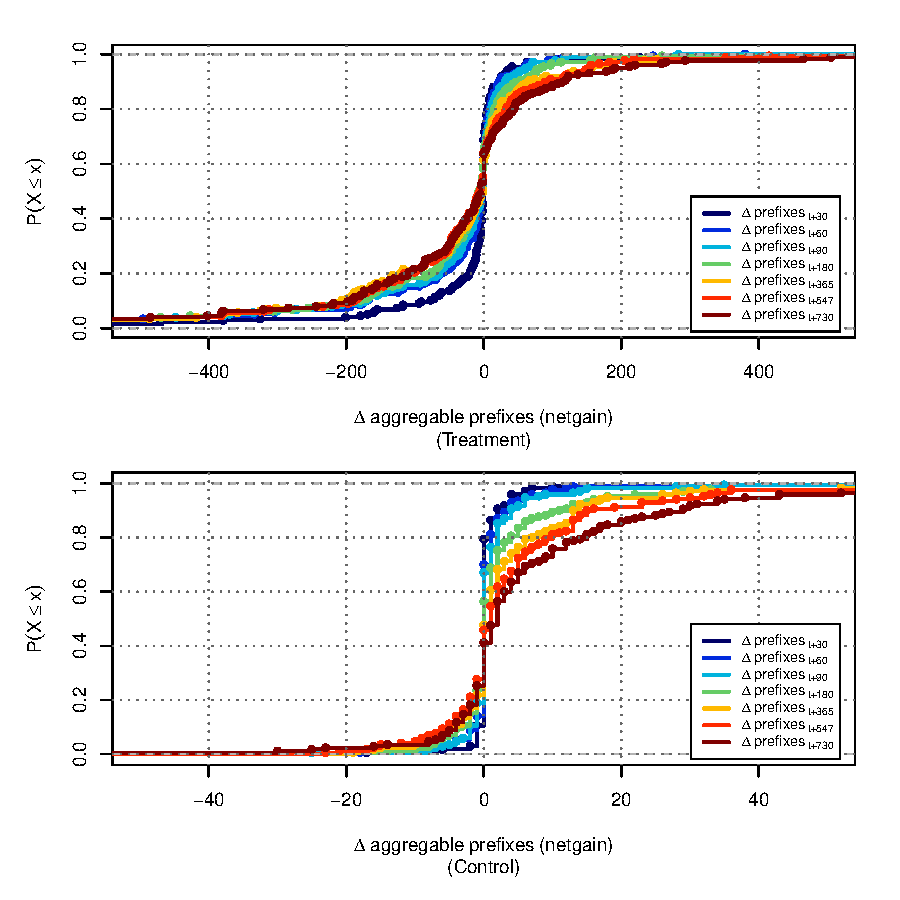
\includegraphics[width=6in]{figures/behavior-netgain-2001_2003-corr.pdf}
    \vspace{-2em}\\
    \caption{Cumulative distribution function of change in number ofaggregable
    prefixes (netgain) advertised by treated and untreated(control) ASes, for
    the period 2001-2003.}
\end{singlespace}
\end{centering}
\end{figure}

\clearpage
\vspace*{16pt}
\begin{figure}[H]
\begin{centering}
\begin{singlespace}
\captionsetup{list=no}
    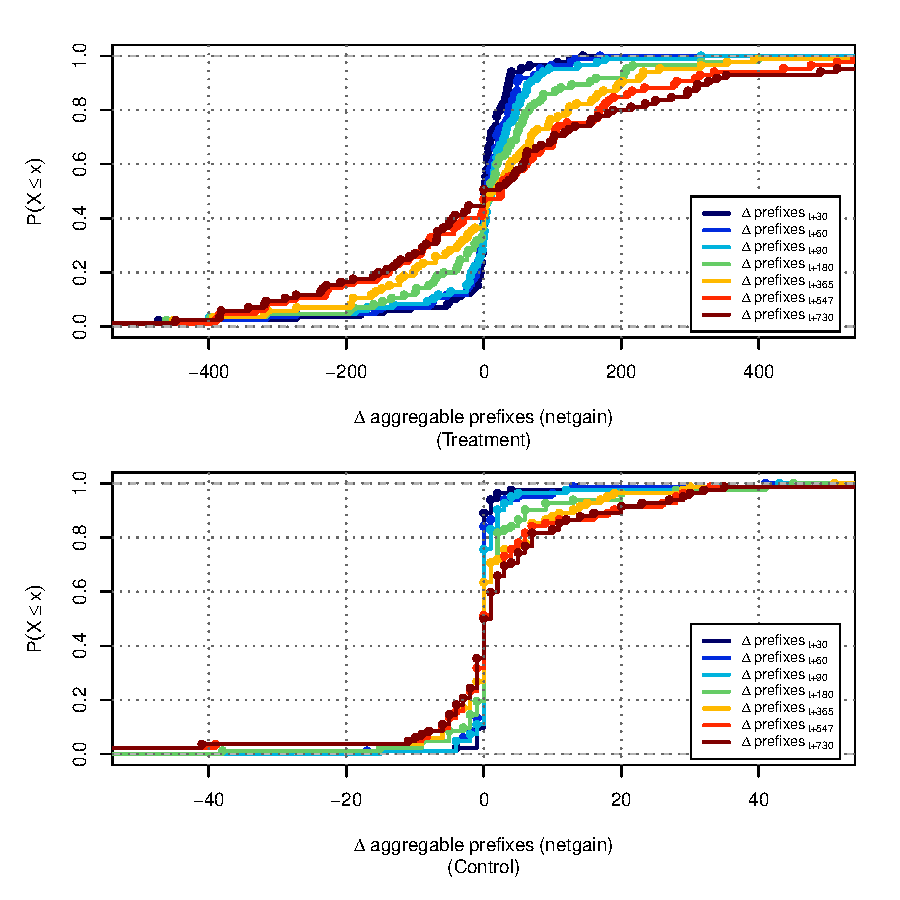
\includegraphics[width=6in]{figures/behavior-netgain-2004_2006-corr.pdf}
    \vspace{-2em}\\
    \caption{Cumulative distribution function of change in number ofaggregable
    prefixes (netgain) advertised by treated and untreated(control) ASes, for
    the period 2004-2006.}
\end{singlespace}
\end{centering}
\end{figure}

\clearpage
\vspace*{16pt}
\begin{figure}[H]
\begin{centering}
\begin{singlespace}
\captionsetup{list=no}
    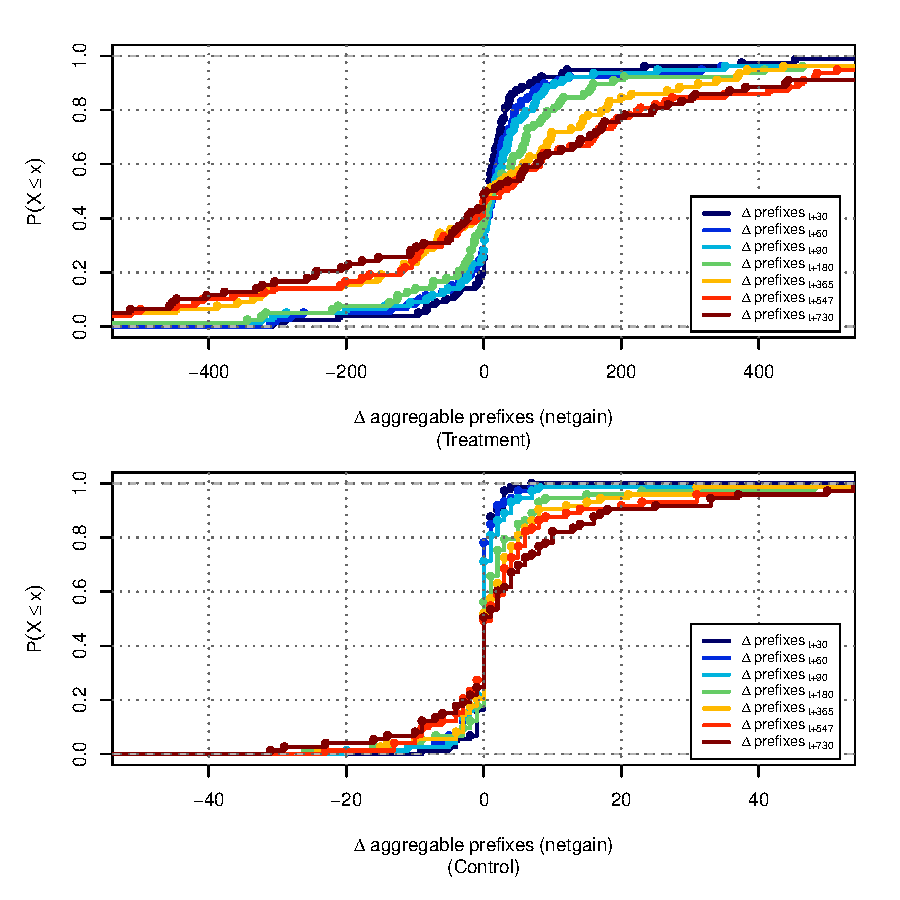
\includegraphics[width=6in]{figures/behavior-netgain-2007_2009-corr.pdf}
    \vspace{-2em}\\
    \caption{Cumulative distribution function of change in number ofaggregable
    prefixes (netgain) advertised by treated and untreated(control) ASes, for
    the period 2007-2009.}
\end{singlespace}
\end{centering}
\end{figure}


%%%%%%%%%%%%%%%%%%%%%%%%%%%%%%%%%%%%%%%%%%%%%%%%%%%%%%%%%%%%%%%%%%%%%%%%%%%%%%%%
\clearpage
\section{Relative netgain}

\begin{figure}[H]
\begin{centering}
\begin{singlespace}
\captionsetup{list=no}
    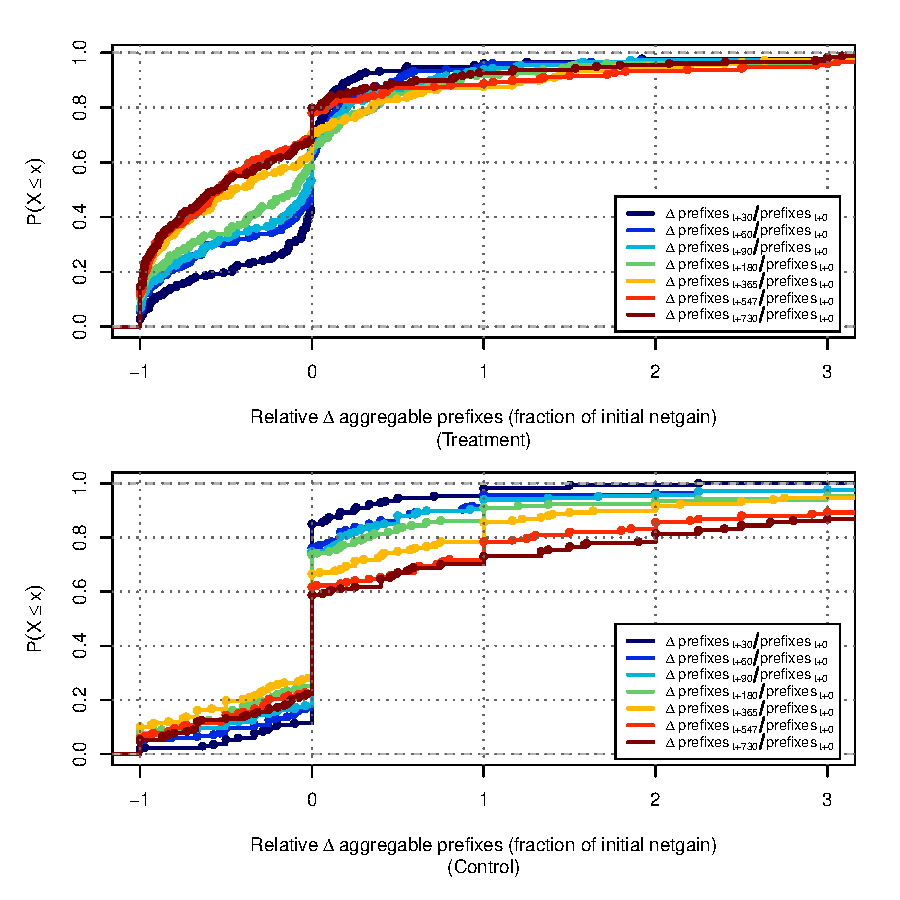
\includegraphics[width=6in]{figures/behavior-rel_netgain-1998_2000-corr.pdf}
    \vspace{-2em}\\
    \caption{Cumulative distribution function of relative change in number of
    aggregable prefixes (netgain) advertised by treated and untreated (control)
    ASes, for the period 1998-2000.}
\end{singlespace}
\end{centering}
\end{figure}

\clearpage
\vspace*{16pt}
\begin{figure}[H]
\begin{centering}
\begin{singlespace}
\captionsetup{list=no}
    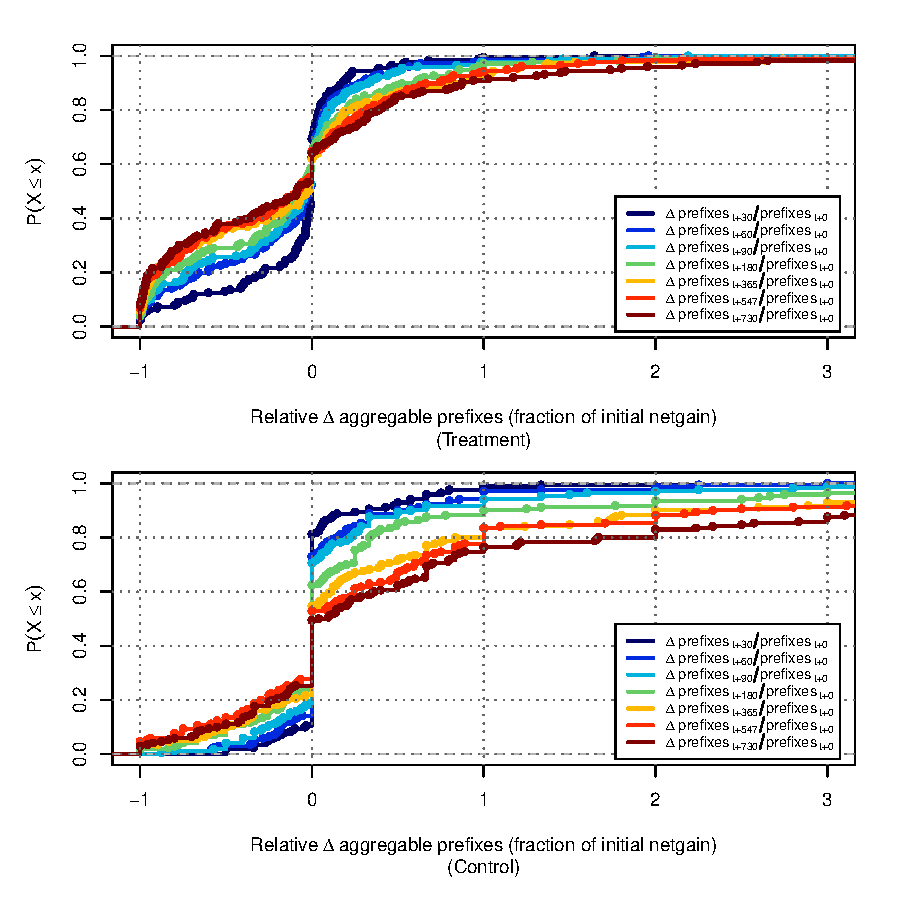
\includegraphics[width=6in]{figures/behavior-rel_netgain-2001_2003-corr.pdf}
    \vspace{-2em}\\
    \caption{Cumulative distribution function of relative change in number of
    aggregable prefixes (netgain) advertised by treated and untreated (control)
    ASes, for the period 2001-2003.}
\end{singlespace}
\end{centering}
\end{figure}

\clearpage
\vspace*{16pt}
\begin{figure}[H]
\begin{centering}
\begin{singlespace}
\captionsetup{list=no}
    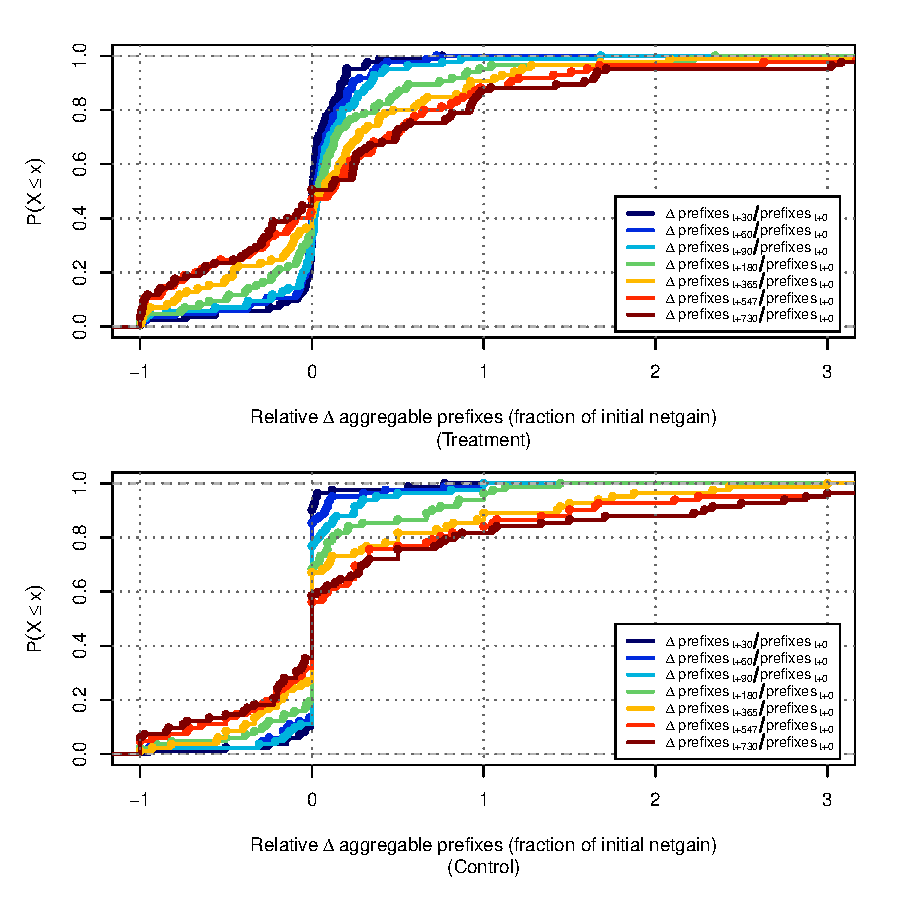
\includegraphics[width=6in]{figures/behavior-rel_netgain-2004_2006-corr.pdf}
    \vspace{-2em}\\
    \caption{Cumulative distribution function of relative change in number of
    aggregable prefixes (netgain) advertised by treated and untreated (control)
    ASes, for the period 2004-2006.}
\end{singlespace}
\end{centering}
\end{figure}

\clearpage
\vspace*{16pt}
\begin{figure}[H]
\begin{centering}
\begin{singlespace}
\captionsetup{list=no}
    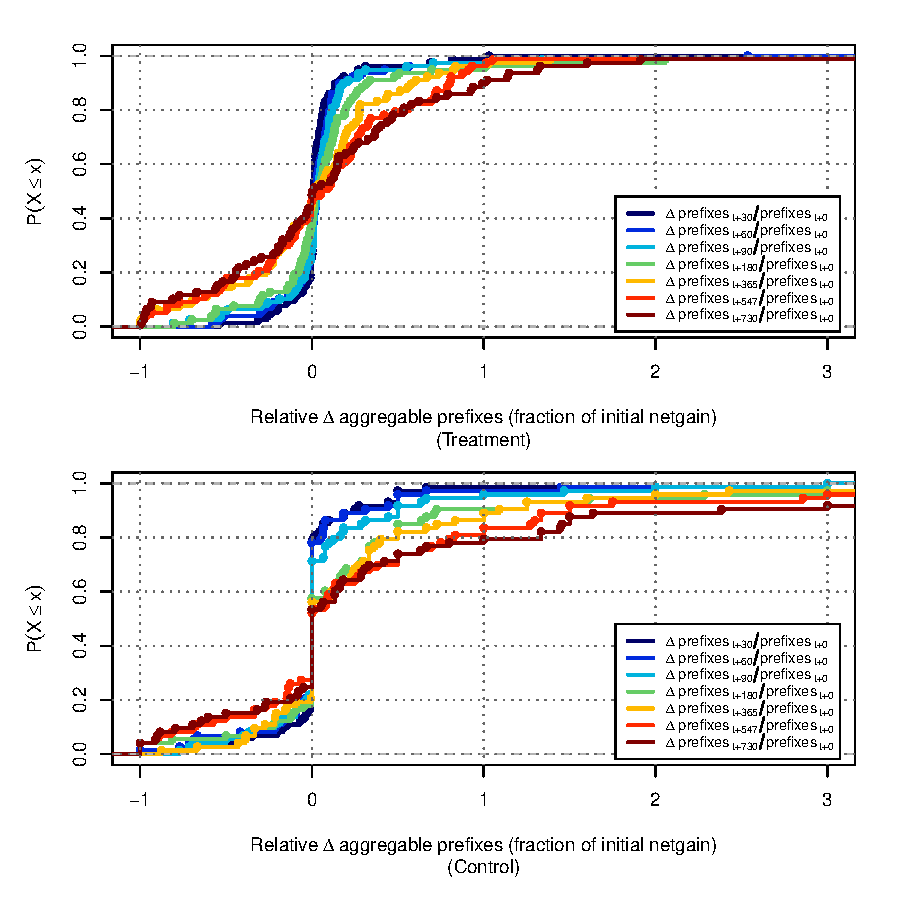
\includegraphics[width=6in]{figures/behavior-rel_netgain-2007_2009-corr.pdf}
    \vspace{-2em}\\
    \caption{Cumulative distribution function of relative change in number of
    aggregable prefixes (netgain) advertised by treated and untreated (control)
    ASes, for the period 2007-2009.}
\end{singlespace}
\end{centering}
\end{figure}

%%% special figures

\clearpage
\begin{figure}[H]
\begin{centering}
\begin{singlespace}
\captionsetup{list=no}
    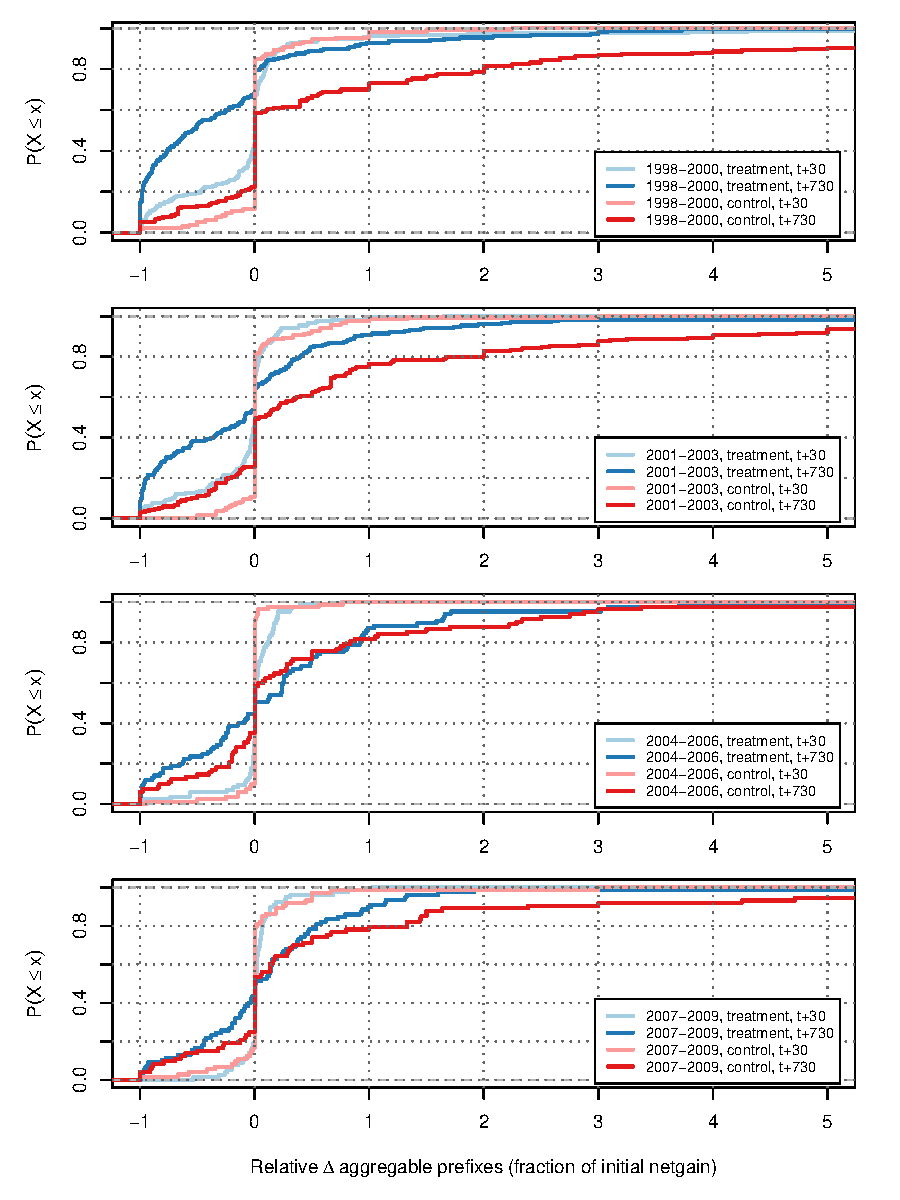
\includegraphics[width=6in]
        {figures/behavior-rel_netgain-vseries-special_tc.pdf}
    \vspace{-2em}\\
    \caption{Simplified relative netgain CDFs for four three-year time
    periods over the full data availability period. In all cases, the the data
    ranges from the first CIDR Report of the ending year until the last CIDR
    Report of the ending year.}
\end{singlespace}
\end{centering}
\end{figure}

\clearpage
\begin{figure}[H]
\begin{centering}
\begin{singlespace}
\captionsetup{list=no}
    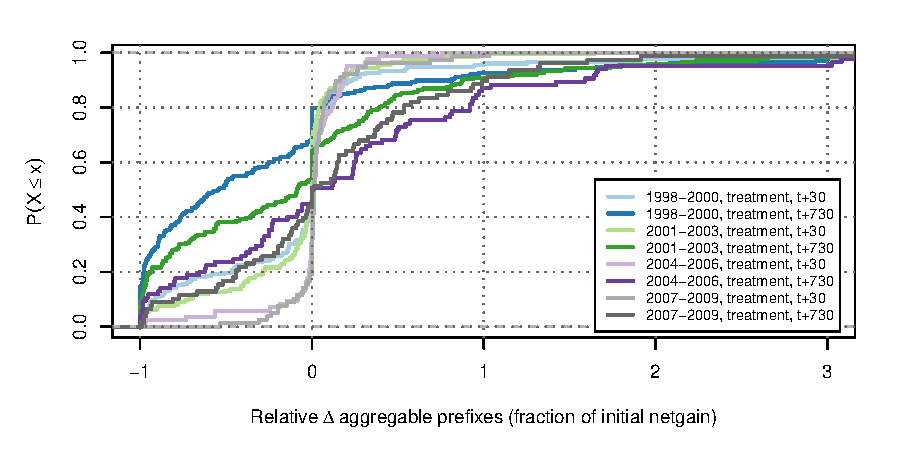
\includegraphics[width=6in]
        {figures/behavior-rel_netgain-all-special_t.pdf}
    \vspace{-2em}\\
    \caption{Superposition of simplified relative netgain CDFs for the
    treated ASes for the four time periods, showing a notable change in
    behavior of ASes appearing on the CIDR Report over time.}
\end{singlespace}
\end{centering}
\end{figure}

\begin{figure}[H]
\begin{centering}
\begin{singlespace}
\captionsetup{list=no}
    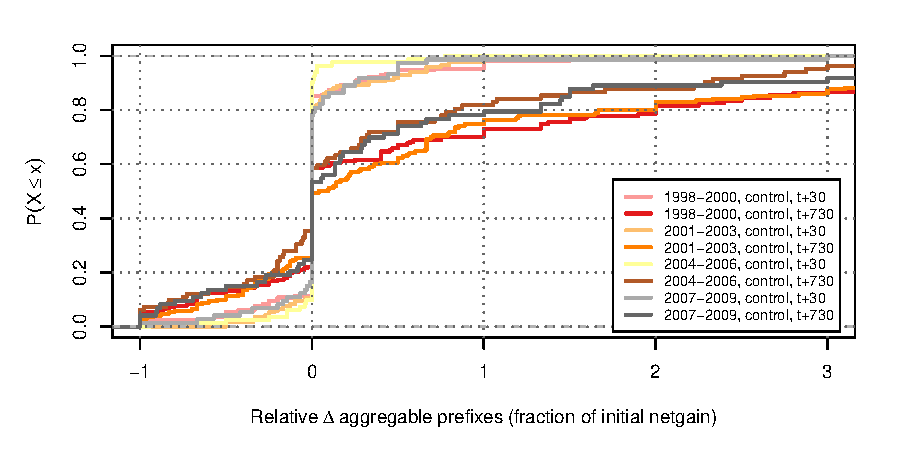
\includegraphics[width=6in]
        {figures/behavior-rel_netgain-all-special_c.pdf}
    \vspace{-2em}\\
    \caption{Superposition of simplified relative netgain CDFs for the
    untreated control ASes for the four time periods, showing generally similar
    behavior of untreated ASes throughout time.}
\end{singlespace}
\end{centering}
\end{figure}

%%%%%%%%%%%%%%%%%%%%%%%%%%%%%%%%%%%%%%%%%%%%%%%%%%%%%%%%%%%%%%%%%%%%%%%%%%%%%%%%
\clearpage
\section{Absolute netsnow}

\begin{figure}[H]
\begin{centering}
\begin{singlespace}
\captionsetup{list=no}
    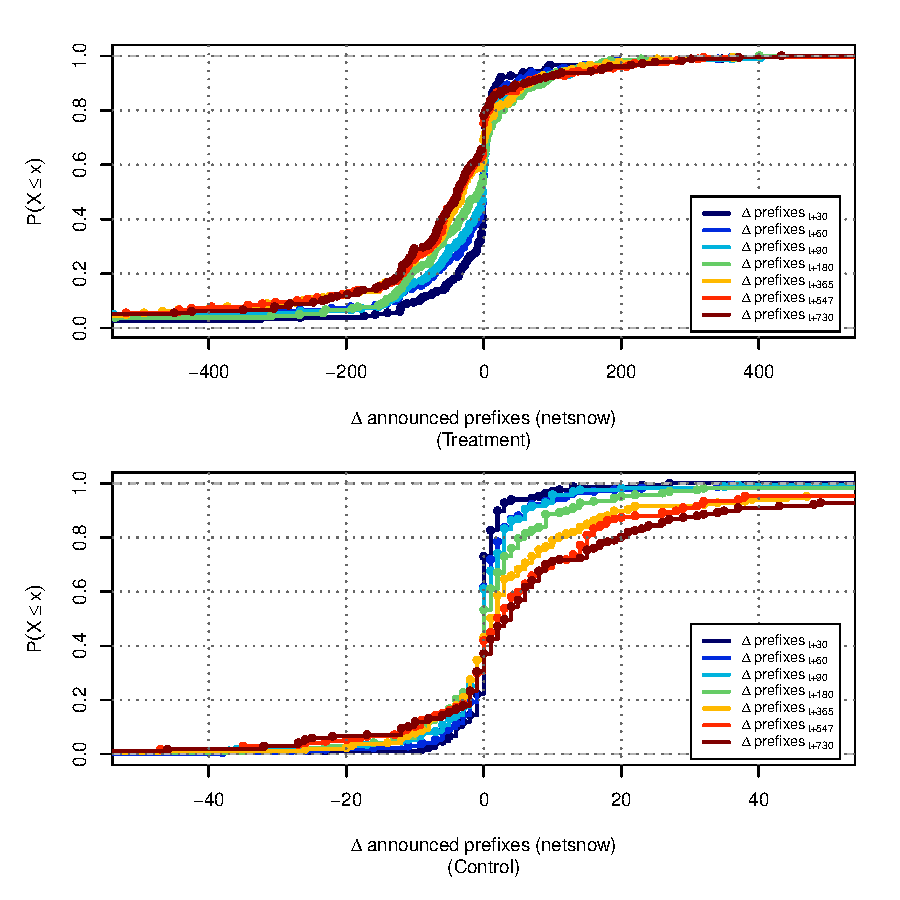
\includegraphics[width=6in]{figures/behavior-netsnow-1998_2000-corr.pdf}
    \vspace{-2em}\\
    \caption{Cumulative distribution function of change in total number of
    prefixes (netsnow) advertised by treated and untreated (control) ASes, for
    the period 1998-2000.}
\end{singlespace}
\end{centering}
\end{figure}

\clearpage
\vspace*{16pt}
\begin{figure}[H]
\begin{centering}
\begin{singlespace}
\captionsetup{list=no}
    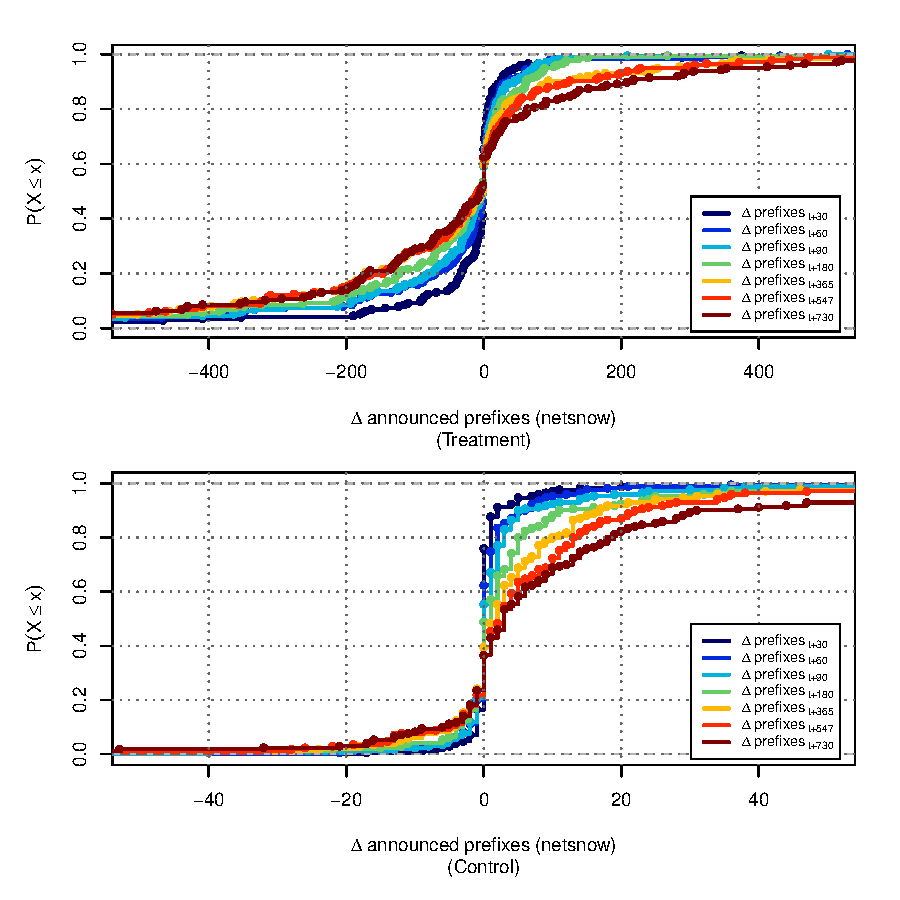
\includegraphics[width=6in]{figures/behavior-netsnow-2001_2003-corr.pdf}
    \vspace{-2em}\\
    \caption{Cumulative distribution function of change in total number of
    prefixes (netsnow) advertised by treated and untreated (control) ASes, for
    the period 2001-2003.}
\end{singlespace}
\end{centering}
\end{figure}

\clearpage
\vspace*{16pt}
\begin{figure}[H]
\begin{centering}
\begin{singlespace}
\captionsetup{list=no}
    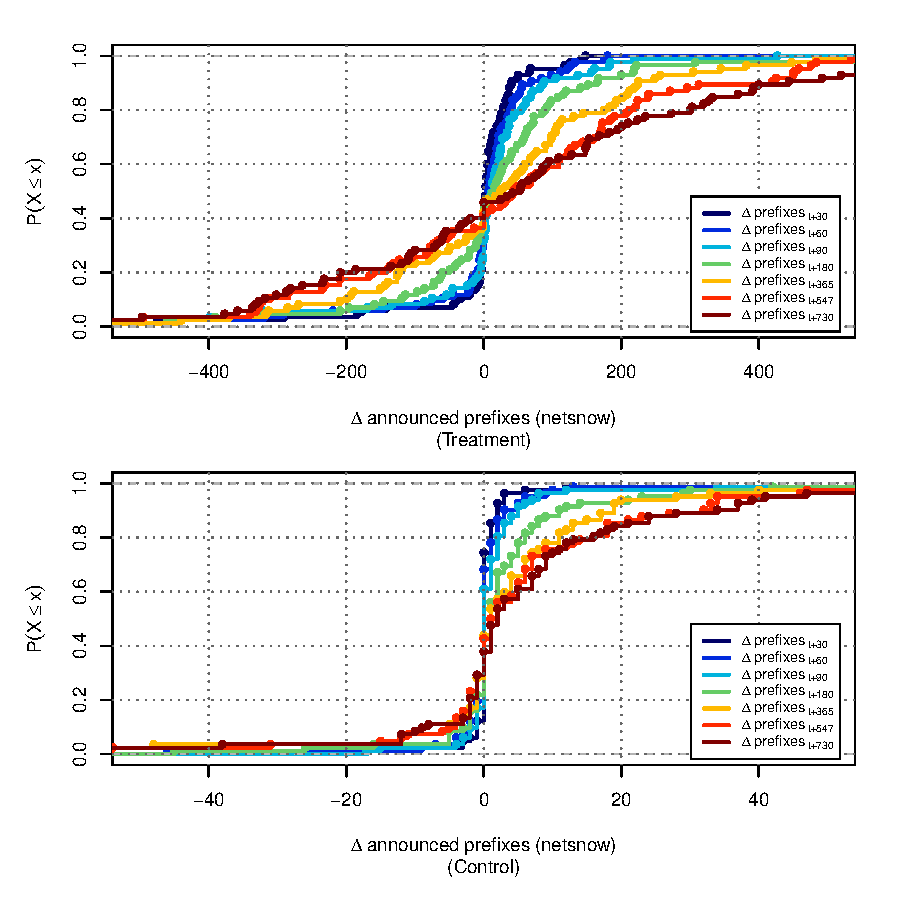
\includegraphics[width=6in]{figures/behavior-netsnow-2004_2006-corr.pdf}
    \vspace{-2em}\\
    \caption{Cumulative distribution function of change in total number of
    prefixes (netsnow) advertised by treated and untreated (control) ASes, for
    the period 2004-2006.}
\end{singlespace}
\end{centering}
\end{figure}

\clearpage
\vspace*{16pt}
\begin{figure}[H]
\begin{centering}
\begin{singlespace}
\captionsetup{list=no}
    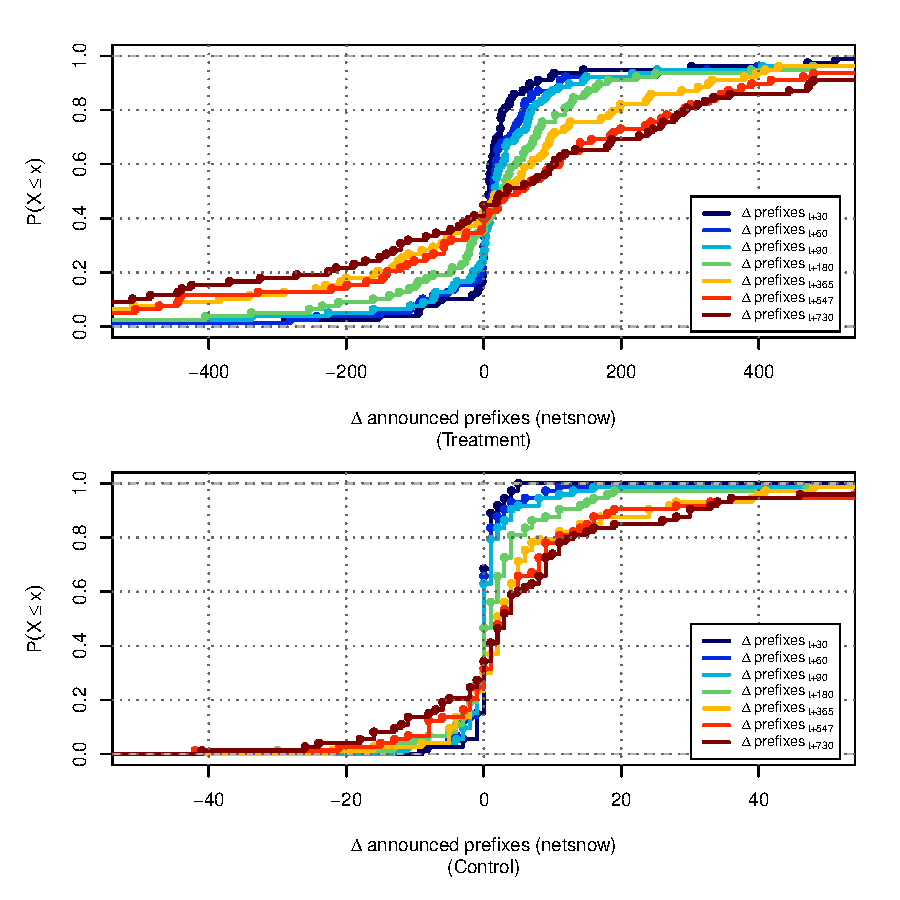
\includegraphics[width=6in]{figures/behavior-netsnow-2007_2009-corr.pdf}
    \vspace{-2em}\\
    \caption{Cumulative distribution function of change in total number of
    prefixes (netsnow) advertised by treated and untreated (control) ASes, for
    the period 2007-2009.}
\end{singlespace}
\end{centering}
\end{figure}


%%%%%%%%%%%%%%%%%%%%%%%%%%%%%%%%%%%%%%%%%%%%%%%%%%%%%%%%%%%%%%%%%%%%%%%%%%%%%%%%
\clearpage
\section{Relative netsnow}

\begin{figure}[H]
\begin{centering}
\begin{singlespace}
\captionsetup{list=no}
    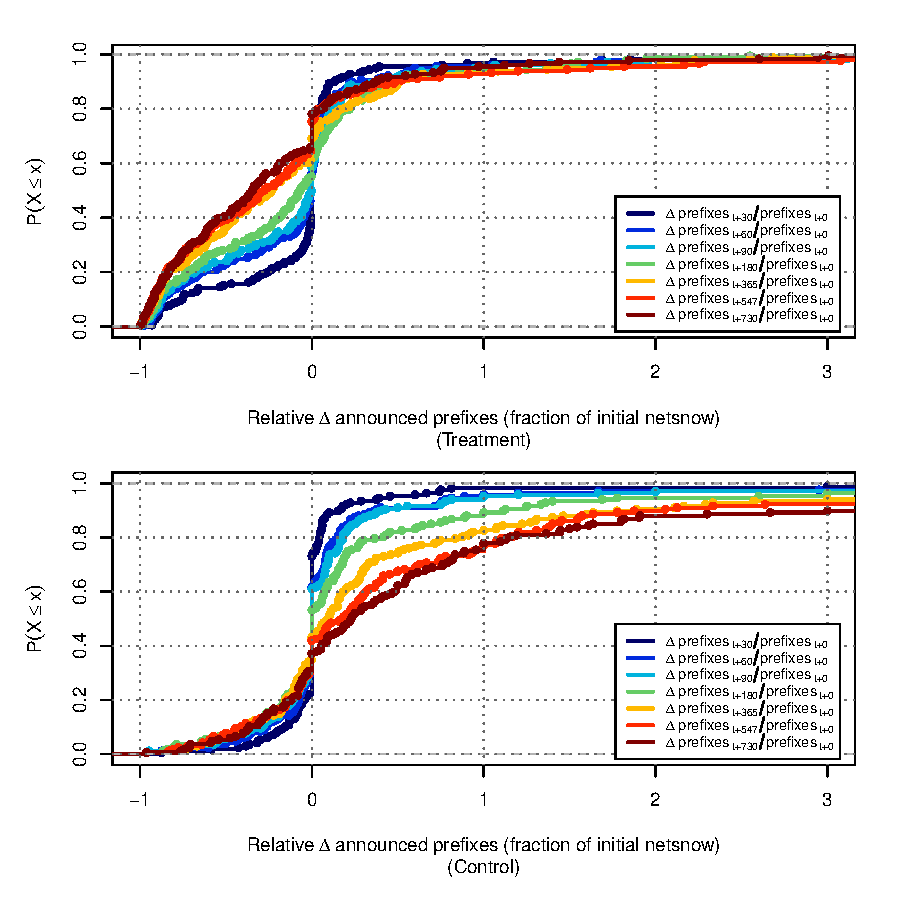
\includegraphics[width=6in]{figures/behavior-rel_netsnow-1998_2000-corr.pdf}
    \vspace{-2em}\\
    \caption{Cumulative distribution function of relative change in total
    number of prefixes (netsnow) advertised by treated and untreated (control)
    ASes, for the period 1998-2000.}
\end{singlespace}
\end{centering}
\end{figure}

\clearpage
\vspace*{16pt}
\begin{figure}[H]
\begin{centering}
\begin{singlespace}
\captionsetup{list=no}
    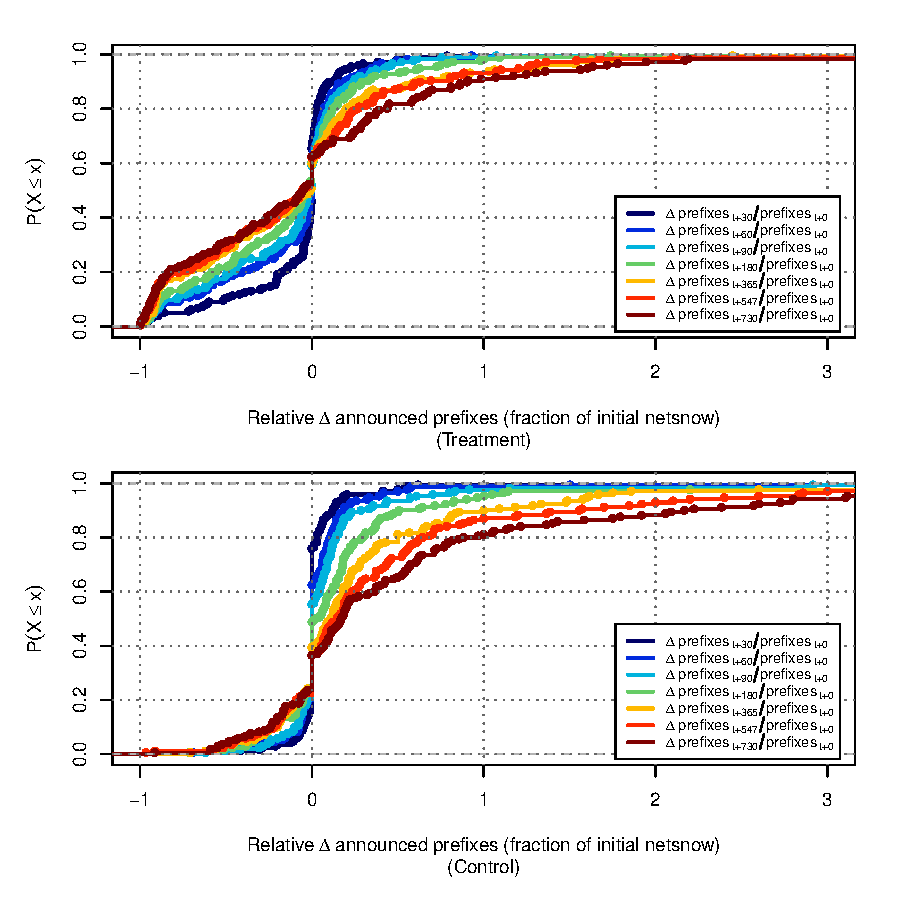
\includegraphics[width=6in]{figures/behavior-rel_netsnow-2001_2003-corr.pdf}
    \vspace{-2em}\\
    \caption{Cumulative distribution function of relative change in total
    number of prefixes (netsnow) advertised by treated and untreated (control)
    ASes, for the period 2001-2003.}
\end{singlespace}
\end{centering}
\end{figure}

\clearpage
\vspace*{16pt}
\begin{figure}[H]
\begin{centering}
\begin{singlespace}
\captionsetup{list=no}
    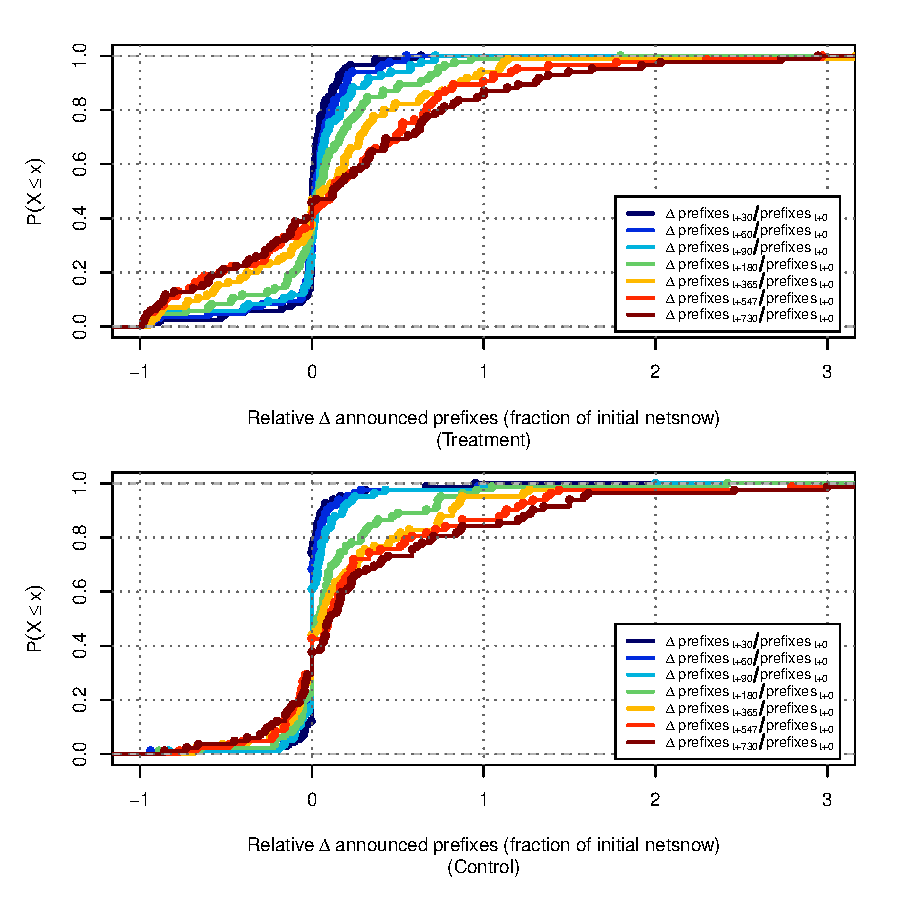
\includegraphics[width=6in]{figures/behavior-rel_netsnow-2004_2006-corr.pdf}
    \vspace{-2em}\\
    \caption{Cumulative distribution function of relative change in total
    number of prefixes (netsnow) advertised by treated and untreated (control)
    ASes, for the period 2004-2006.}
\end{singlespace}
\end{centering}
\end{figure}

\clearpage
\vspace*{16pt}
\begin{figure}[H]
\begin{centering}
\begin{singlespace}
\captionsetup{list=no}
    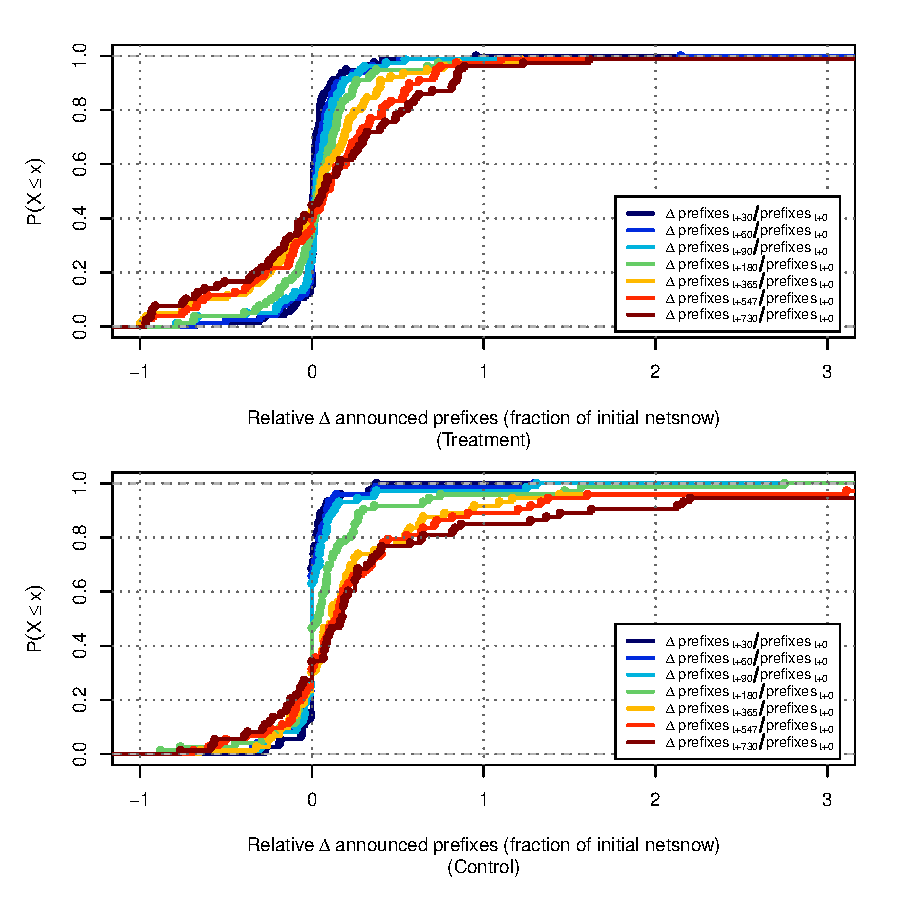
\includegraphics[width=6in]{figures/behavior-rel_netsnow-2007_2009-corr.pdf}
    \vspace{-2em}\\
    \caption{Cumulative distribution function of relative change in total
    number of prefixes (netsnow) advertised by treated and untreated (control)
    ASes, for the period 2007-2009.}
\end{singlespace}
\end{centering}
\end{figure}


%%%%%%%%%%%%%%%%%%%%%%%%%%%%%%%%%%%%%%%%%%%%%%%%%%%%%%%%%%%%%%%%%%%%%%%%%%%%%%%%
% \clearpage
% \section{Fraction Aggregable}
%
% \begin{figure}[H]
% \begin{centering}
% \begin{singlespace}
% \captionsetup{list=no}
%     \includegraphics[width=6in]
%     {figures/behavior-frac_deagg-1997_2011-corr.pdf}
%     \vspace{-2em}\\
%     \caption{Cumulative distribution function of the fraction of prefixes
%     announced by each AS that are aggregable, for both treated and untreated
%     (control) ASes, for the period 1997-2011. This figure is for the entire
%     period, instead of particular slots, and was included to be congruent with
%     the full-period figures for other quantities included in the body of the
%     thesis.}
% \end{singlespace}
% \end{centering}
% \end{figure}
%
%
% \clearpage
% \vspace*{16pt}
% \begin{figure}[H]
% \begin{centering}
% \begin{singlespace}
% \captionsetup{list=no}
%     \includegraphics[width=6in]
%     {figures/behavior-frac_deagg-1998_2000-corr.pdf}
%     \vspace{-2em}\\
%     \caption{Cumulative distribution function of change in the fraction of
%     prefixes advertised by treated and untreated (control) ASes that can be
%     aggregated without affecting routing policy, for the period 1998-2000.}
% \end{singlespace}
% \end{centering}
% \end{figure}
%
% \clearpage
% \vspace*{16pt}
% \begin{figure}[H]
% \begin{centering}
% \begin{singlespace}
% \captionsetup{list=no}
%     \includegraphics[width=6in]
%     {figures/behavior-frac_deagg-2001_2003-corr.pdf}
%     \vspace{-2em}\\
%     \caption{Cumulative distribution function of change in the fraction of
%     prefixes advertised by treated and untreated (control) ASes that can be
%     aggregated without affecting routing policy, for the period 2001-2003.}
% \end{singlespace}
% \end{centering}
% \end{figure}
%
% \clearpage
% \vspace*{16pt}
% \begin{figure}[H]
% \begin{centering}
% \begin{singlespace}
% \captionsetup{list=no}
%     \includegraphics[width=6in]
%     {figures/behavior-frac_deagg-2004_2006-corr.pdf}
%     \vspace{-2em}\\
%     \caption{Cumulative distribution function of change in the fraction of
%     prefixes advertised by treated and untreated (control) ASes that can be
%     aggregated without affecting routing policy, for the period 2004-2006.}
% \end{singlespace}
% \end{centering}
% \end{figure}
%
% \clearpage
% \vspace*{16pt}
% \begin{figure}[H]
% \begin{centering}
% \begin{singlespace}
% \captionsetup{list=no}
%     \includegraphics[width=6in]
%     {figures/behavior-frac_deagg-2007_2009-corr.pdf}
%     \vspace{-2em}\\
%     \caption{Cumulative distribution function of change in the fraction of
%     prefixes advertised by treated and untreated (control) ASes that can be
%     aggregated without affecting routing policy, for the period 2007-2009.}
% \end{singlespace}
% \end{centering}
% \end{figure}
%
%
%%%%%%%%%%%%%%%%%%%%%%%%%%%%%%%%%%%%%%%%%%%%%%%%%%%%%%%%%%%%%%%%%%%%%%%%%%%%%%%%
\clearpage
\section{Deaggregation Factor}

\begin{figure}[H]
\begin{centering}
\begin{singlespace}
\captionsetup{list=no}
    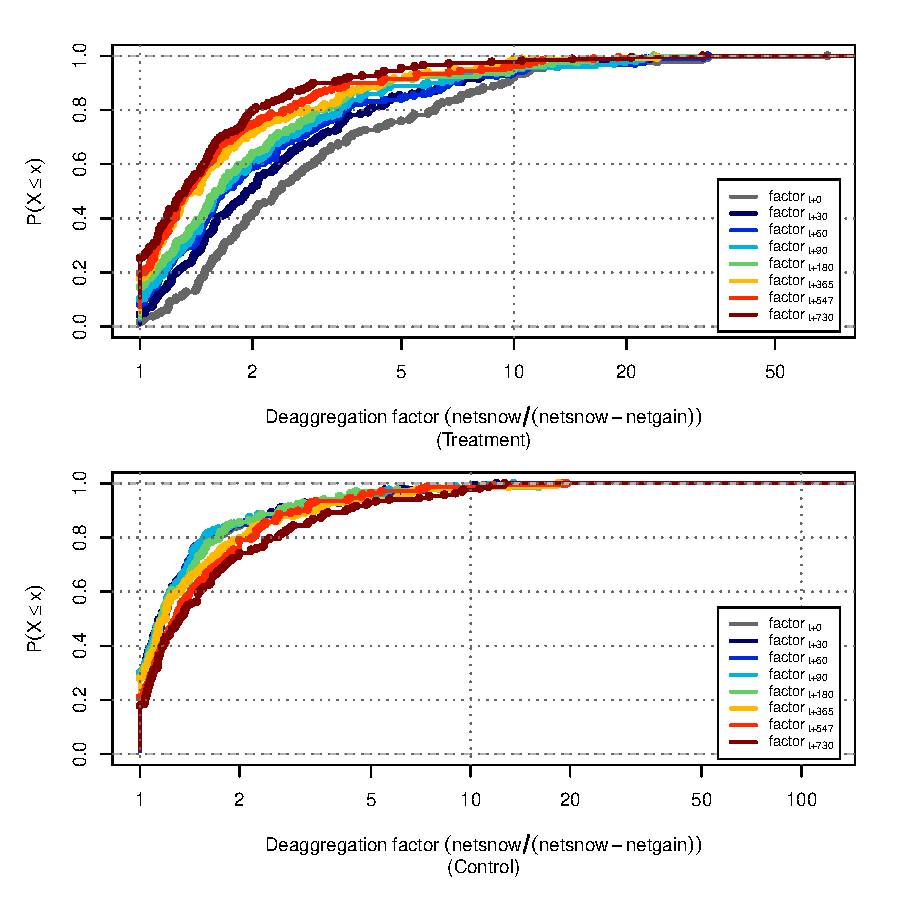
\includegraphics[width=6in]
    {figures/behavior-deagg_factor-1998_2000-corr.pdf}
    \vspace{-2em}\\
    \caption{Cumulative distribution function of change in the deaggregation
    factor, the ratio of currently advertised prefixes to perfectly aggregated
    prefixes, of treated and untreated (control) ASes, for the period
    1998-2000.}
\end{singlespace}
\end{centering}
\end{figure}

\clearpage
\vspace*{16pt}
\begin{figure}[H]
\begin{centering}
\begin{singlespace}
\captionsetup{list=no}
    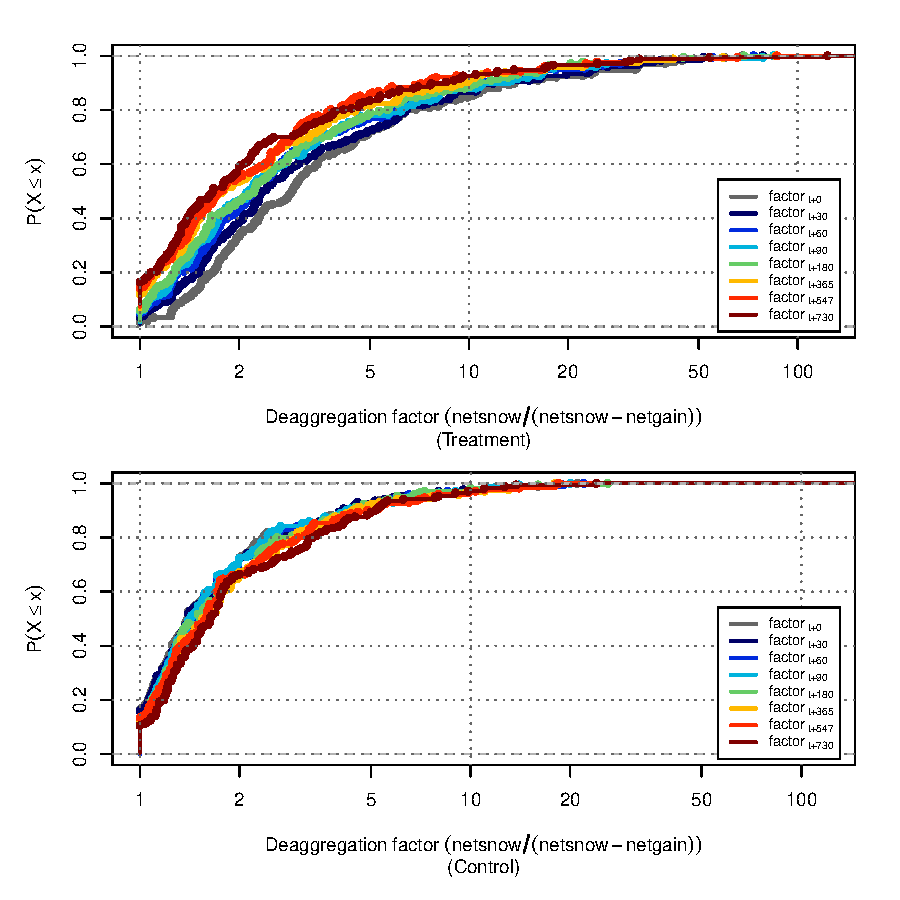
\includegraphics[width=6in]
    {figures/behavior-deagg_factor-2001_2003-corr.pdf}
    \vspace{-2em}\\
    \caption{Cumulative distribution function of change in the deaggregation
    factor, the ratio of currently advertised prefixes to perfectly aggregated
    prefixes, of treated and untreated (control) ASes, for the period
    2001-2003.}
\end{singlespace}
\end{centering}
\end{figure}

\clearpage
\vspace*{16pt}
\begin{figure}[H]
\begin{centering}
\begin{singlespace}
\captionsetup{list=no}
    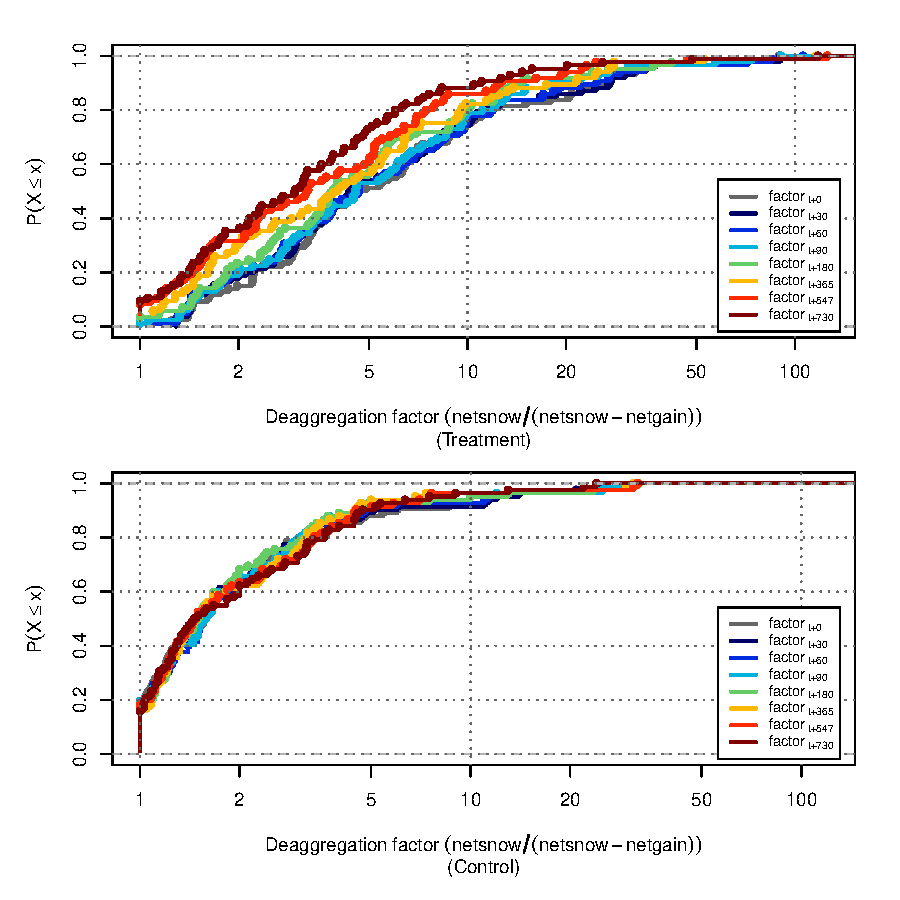
\includegraphics[width=6in]
    {figures/behavior-deagg_factor-2004_2006-corr.pdf}
    \vspace{-2em}\\
    \caption{Cumulative distribution function of change in the deaggregation
    factor, the ratio of currently advertised prefixes to perfectly aggregated
    prefixes, of treated and untreated (control) ASes, for the period
    2004-2006.}
\end{singlespace}
\end{centering}
\end{figure}

\clearpage
\vspace*{16pt}
\begin{figure}[H]
\begin{centering}
\begin{singlespace}
\captionsetup{list=no}
    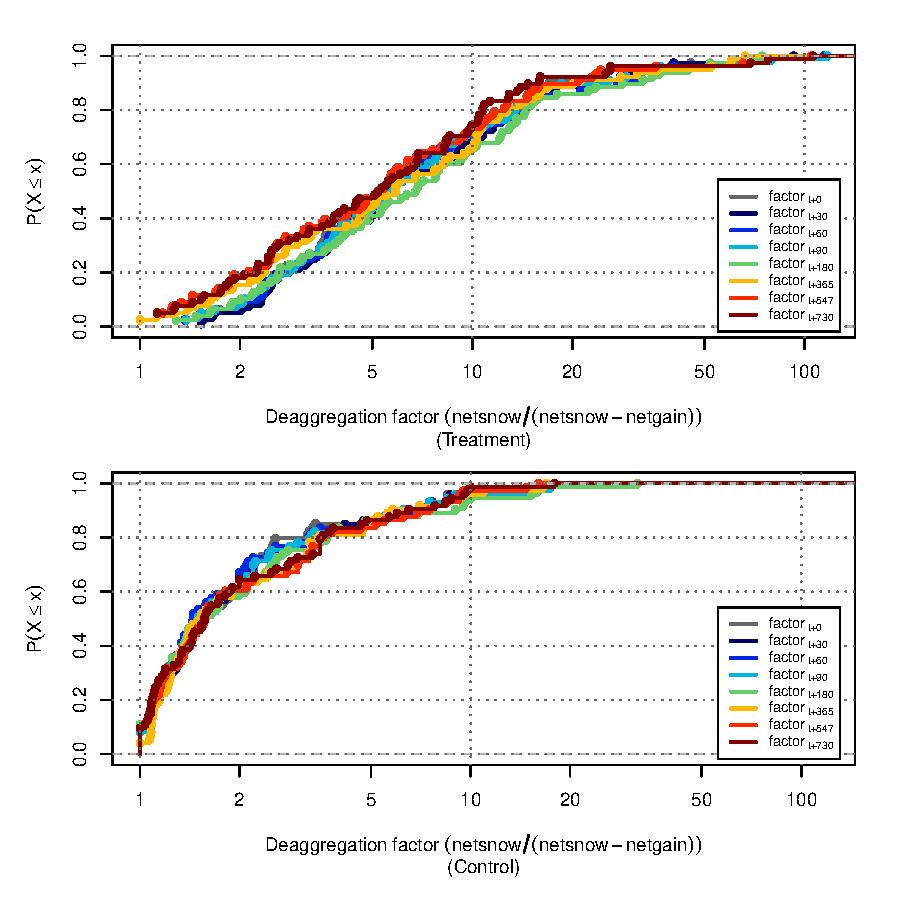
\includegraphics[width=6in]
    {figures/behavior-deagg_factor-2007_2009-corr.pdf}
    \vspace{-2em}\\
    \caption{Cumulative distribution function of change in the deaggregation
    factor, the ratio of currently advertised prefixes to perfectly aggregated
    prefixes, of treated and untreated (control) ASes, for the period
    2007-2009.}
\end{singlespace}
\end{centering}
\end{figure}

